\documentclass{book}
\usepackage{hyperref}
\usepackage{geometry}
\usepackage{graphicx}
\usepackage{apacite}
\usepackage{natbib}
\usepackage{float}
\usepackage{subfigure}
\usepackage{array,booktabs} % Table packages

\hypersetup{
    colorlinks=true,
    linkcolor=black,
    filecolor=magenta,      
    urlcolor=cyan,
    pdftitle={Sharelatex Example},
    bookmarks=true,
    pdfpagemode=FullScreen,
}

\pagestyle{empty}
\graphicspath{{img/}}
\begin{document}
    \begin{titlepage}
        \centering
        
\includegraphics[width=6cm]{logo-unipi.png}
        \vfill
        \vspace{1.5cm}
        {\huge\textsc{Computational Intelligence and Deep Learning}\par}
        {\Large
            Educational Version\\
            2020\\
            \vspace{2cm}
            A. Schiavo - M. Gómez - M. Daole \\
            \vspace{2cm}
            \today
        }    
        \vfill
        \vfill
    \end{titlepage}
    \tableofcontents


    % --------------------------------------------------------------------
    \chapter{Introduction}

    Breast cancer is one of the most common types of cancer in women. Early detection and treatment can effectively improve cure rates and reduce mortality. Detecting breast cancer using mammographic images is a cost-effective technique, and radiologists can make a diagnosis by analyzing these images. However, the large number of mammographic images produced day by day has brought a huge workload on radiologists and also increased the rate of misdiagnosis. Therefore, developing a computer-aided diagnosis (CAD) system can significantly relieve the pressure on radiologists and improve the diagnosis accuracy.
    
    Machine learning therefore quickly enters the picture, based on large, heterogeneous data sets, the automatic analysis for mammography images needs to be analyzed and make predictions from the regions of interest and classify these regions into normal or abnormal (benign and malignant).
    
        \section{Notebooks}
        \begin{enumerate}
            \item \textbf{Knowing the Dataset}
            \begin{itemize}
                \item \href{https://github.com/MarshaGomez/CNN-Medical-Imaging-Analysis/blob/main/Code/Knowing_DDSM_dataset.ipynb}{Knowing\_DDSM\_dataset.ipynb}
            \end{itemize}
            \item \textbf{CNN from Scratch}
            \begin{itemize}
                \item \href{https://github.com/MarshaGomez/CNN-Medical-Imaging-Analysis/blob/main/Code/Scratch_CNN_benign_vs_malign.ipynb}{Scratch\_CNN\_benign\_vs\_malign.ipynb}
                \item \href{https://github.com/MarshaGomez/CNN-Medical-Imaging-Analysis/blob/main/Code/ Scratch_CNN_masses_vs_calc.ipynb}{Scratch\_CNN\_masses\_vs\_calc.ipynb}
            \end{itemize}
            \item \textbf{PreTrained}
            \begin{itemize}
                \item \href{https://github.com/MarshaGomez/CNN-Medical-Imaging-Analysis/blob/main/Code/ PreTrained_CNN_benign_vs_malign.ipynb}{PreTrained\_CNN\_benign\_vs\_malign.ipynb}
                \item \href{https://github.com/MarshaGomez/CNN-Medical-Imaging-Analysis/blob/main/Code/ PreTrained_CNN_masses_vs_calc.ipynb}{PreTrained\_CNN\_masses\_vs\_calc.ipynb}
            \end{itemize}
            \item \textbf{Baseline}
            \begin{itemize} 
                \item \href{https://github.com/MarshaGomez/CNN-Medical-Imaging-Analysis/blob/main/Code/ BaselineCNN.ipynb}{BaselineCNN.ipynb}
            \end{itemize}
            \item \textbf{Esemble}
            \begin{itemize} 
                \item \href{https://github.com/MarshaGomez/CNN-Medical-Imaging-Analysis/blob/main/Code/Ensemble.ipynb}{Ensemble.ipynb}
            \end{itemize}
        \end{enumerate}

    % --------------------------------------------------------------------

    \chapter{Convolutional Neural Network for Medical Imaging Analysis}  % -- All the images on this chapter starts with the name Introduction (intro-xxxxx.png) 

    On this investigation, the main objective is to perform abnormality classification in mammography using Convolutional Neural Networks for Medical Imaging Analysis. This laboratory research will be development with a standart evaluation data set in the area of decision support systems in mammography, the \textit{Digital Curated Breast Imaging Subset of Database for Screening Mammography} \textbf{(CBIS DDSM)}
    
        \section{Original Dataset}
        The dataset we will focus on is an updated and standardized version of the Digital Database for Screening Mammography (DDSM). The DDSM is a database of 2,620 scanned film mammography studies. It contains normal, benign, and malignant cases with verified pathology information. Few well-curated public datasets have been provided for the mammography community. These include the DDSM, the Mammographic Imaging Analysis Society (MIAS) database, and the Image Retrieval in Medical Applications (IRMA) project. Although these public data sets are useful, they are limited in terms of data set size and accessibility.

        \begin{center}
            \begin{minipage}{0.9\linewidth}
                \vspace{5pt}%margen superior de minipage
                {\small
                    Lee, Rebecca Sawyer, et al. \textit{'A curated mammography data set for use in computer-aided detection and diagnosis research'} Scientific data 4 (2017): 170177.
                }
                \vspace{5pt}%margen inferior de la minipage
            \end{minipage}
        \end{center}

        The images have been decompressed and converted to DICOM format. Updated ROI segmentation and bounding boxes, and pathologic diagnosis for training data are also included. The data set contains 753 calcification cases and 891 mass cases, providing a data-set size capable of analyzing decision support systems in mammography.

        
        \begin{table}
            \begin{tabular}{m{5cm}m{8cm}}
                \midrule
                \textbf{Design Types} & -Design Types and Parallel group design.  -Feature extraction objective.  -Image processing objective \\
                \midrule
                \textbf{Measurement Type} & Mammography \\ 
                \midrule
                \textbf{Technology Type} & Digital curation \\ 
                \midrule
                \textbf{Factor Type} & Diagnosis \\
                \midrule
                \textbf{Sample Characteristic} & Homo sapiens\\
                \midrule
            \end{tabular}
            \caption{\label{tab:DDSM}DDSM Data Set description.}
        \end{table}

        In the subsequent sections, data source, data preprocessing, data augmentation, model development and evaluation will be delineated. A simple example of the image provided from the original dataset:

        \begin{figure}[H]
            \subfigure[Mass, Benign]{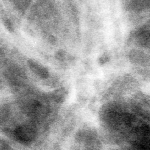
\includegraphics[width=3cm]{intro-masses-benign.png}}
            \hfill
            \subfigure[Mass, Malignant]{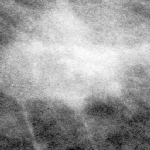
\includegraphics[width=3cm]{intro-masses-malign.png}}
            \hfill
            \subfigure[Calcification, Benign]{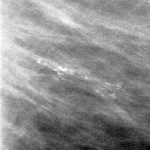
\includegraphics[width=3cm]{intro-calc-benign.png}}
            \hfill
            \subfigure[Calcification, Malignant]{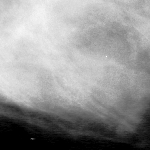
\includegraphics[width=3cm]{intro-calc-malign.png}}
            \hfill
            \caption{Medical Image Representation}
        \end{figure}

        Considering the benefits of using deep learning in image classification problem (e.g., automatic feature extraction from raw data), develop a deep Convolutional Neural Network (CNN) that will be trained to read mammography images and classify them into the following five instances:

        \begin{itemize}
            \item Normal
            \item Benign Calcification
            \item Benign Mass
            \item Malignant Calcification
            \item Malignant Mass
        \end{itemize}
         
        \section{Data Records}
        The images are distributed at the full mammography and abnormality level as DICOM files. Full mammography images include both MLO and CC views of the mammograms. Abnormalities are represented as binary mask images of the same size as their associated
        mammograms. 

        \begin{figure}[h]
            \subfigure[Classes: Baseline patch \textit{(0)}, Mass, benign (1), Mass, malignant \textit{(2)}, Calcification, benign \textit{(3)}, Calcification, malignant \textit{(4)}]{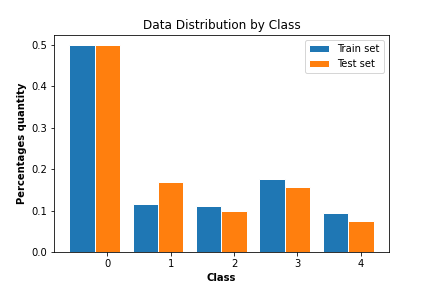
\includegraphics[width=7cm]{intro-dataset-class.png}}
            \hfill
            \subfigure[Pathology: Benign \textit{(0)}, Malignant \textit{(1)}]{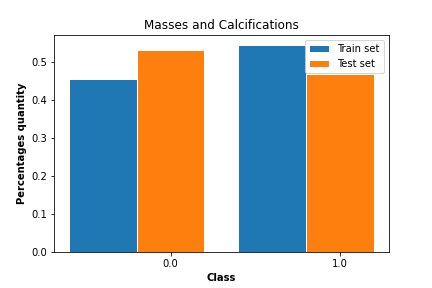
\includegraphics[width=7cm]{intro-dataset-calc-mass.png}}
            \hfill 
            \subfigure[Pathology: Benign \textit{(0)}, Malignant \textit{(1)}]{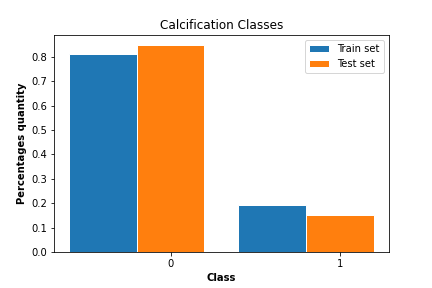
\includegraphics[width=7cm]{intro-dataset-calc.png}}
            \hfill 
            \subfigure[Pathology: Benign \textit{(0)}, Malignant \textit{(1)}]{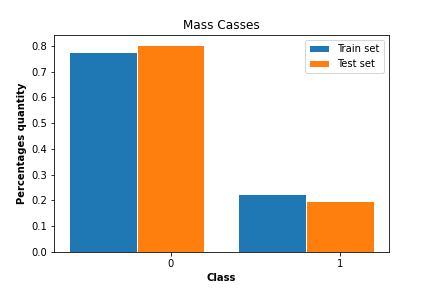
\includegraphics[width=7cm]{intro-dataset-masses.png}}
            \hfill
            \caption{Data Representation}
        \end{figure}

    
    As we mention previously,  \textit{CBIS DDSM:} Curated Breast Imaging Subset of Digital Database for Screening Mammography.

    A description of the dataset is provided in:

    % --------------------------------------------------------------------

    \chapter{CNN from Scratch with Python}
    
        \section{Masses and Calcifications} % -- All the images on this section starts with the name Scratch Masses and Calcifications (smc-xxxxx.png) 

            \subsection{Data Preparation}

            \begin{itemize}
                \item Data Loading
                \item Data Reshape
                \item Data Normalization
                \item Splitting into Training and Validation data
            \end{itemize}

            This can be easily done with the Python data manipulation. Modern deep learning provides a very powerful framework for supervised learning, we introduce on this step the convolutional network for scaling to large images.

            \subsection{Building CNN Architecture}

            \begin{itemize}
                \item Definition CNN Model
                \item Data Optimizer
                
                \begin{table}
                    \begin{center}
                        \begin{tabular}{m{1.8cm}m{1.8cm}m{1cm}m{1.5cm}m{1cm}m{1.3cm}m{1.3cm}m{1cm}m{1cm}}
                            \midrule
                            \textbf{Test Num} & \textbf{Batch size} &	\textbf{Epochs}	& \textbf{Optimizer} &	\textbf{Loss}	& \textbf{Accuracy} &	\textbf{Precision}	& \textbf{Recall}	& \textbf{AUC} \\
                            \midrule
                            \textbf{1} & 20 &	100	& RMSprop & 0.7444	& 0.8313	& 0.8519	& 0.7718	& 0.8803 \\
                            \midrule
                            \textbf{2} & 20 &	100	& Adam & 0.8893	& 0.8031	& 0.7829	& 0.7987	& 0.8761 \\
                            \midrule
                            \textbf{3} & 20 &	100	& Nadam & 0.7338	& 0.8156	& 0.7885	& 0.8255	& 0.9022 \\
                            \midrule
                        \end{tabular}
                    \end{center}
                    \caption{\label{tab:optimizer}Comparation Optimizer}
                \end{table}
            \end{itemize}

            \subsection{Visualization of the Data}
            \subsection{Fighting Overfitting}

            \begin{itemize}
                \item CNN Model No.1 Data Augmentation
                \item CNN Model No.2 K-fold cross validation
            \end{itemize}

            \subsection{Hyperparameter Tuning}

            \begin{table}
                \begin{center}
                    \begin{tabular}{m{1cm}m{1cm}m{2.5cm}m{1.3cm}m{1cm}m{2cm}m{2cm}m{1cm}}
                        \midrule
                        batch size	& num epochs	& units per layer	& optimizer	& learning rate	& mean val acc	& mean val loss	& num folds \\
                        20	& 100	& [32  64  128  128]	& RMSprop	& 0.01	& 0.8615 & 0.3377 & 5 \\
                        \midrule
                        20	& 100	& [32  64  128  256]	& RMSprop	& 0.01	& 0.8777 & 0.3445 & 5 \\
                        \midrule
                        20	& 100	& [32  64  128  128]	& Adam	& 0.01	& 0.8746 & 0.3198 & 5 \\
                        \midrule
                        20	& 100	& [32  64  128  256]	& Adam	& 0.01	& 0.8712 & 0.3218 & 5 \\
                        \midrule
                        20	& 100	& [32  64  128  128]	& RMSprop	& 0.001	& 0.8865 & 0.3032 & 5 \\
                        \midrule
                        20	& 100	& [32  64  128  256]	& RMSprop	& 0.001	& 0.8865 & 0.3096 & 5 \\
                        \midrule
                        20	& 100	& [32  64  128  128]	& Adam	& 0.001	& 0.8808 & 0.3143 & 5 \\
                        \midrule
                        20	& 100	& [32  64  128  256]	& Adam	& 0.001	& 0.8719 & 0.3136 & 5 \\
                        \midrule
                        20	& 100	& [32  64  128  128]	& RMSprop	& 0.0001	& 0.8796 & 0.3183 & 5 \\
                        \midrule
                        20	& 100	& [32  64  128  256]	& RMSprop	& 0.0001	& 0.8704 & 0.3300 & 5 \\
                        \midrule
                        20	& 100	& [32  64  128  128]	& Adam	& 0.0001	& 0.8815 & 0.3031 & 5 \\
                        \midrule
                        20	& 100	& [32  64  128  256]	& Adam	& 0.0001	& 0.8554 & 0.3688 & 5 \\
                        \midrule
                    \end{tabular}
                \end{center}
                \caption{\label{tab:optimizer}Comparation Optimizer}
            \end{table}

            \begin{table}
                \begin{center}
                    \begin{tabular}{m{1cm}m{1cm}m{2.5cm}m{1.3cm}m{1cm}m{2cm}m{2cm}m{1cm}}
                        \midrule
                        batch size	& num epochs	& units per layer	& optimizer	& learning rate	& mean val acc	& mean val loss	& num folds \\
                        \midrule
                        32	& 100	& [32  64  128  128]	& RMSprop	& 0.01	& 0.8609 & 0.3520 & 5 \\
                        \midrule
                        32	& 100	& [32  64  128  256]	& RMSprop	& 0.01	& 0.8723 & 0.3259 & 5 \\
                        \midrule
                        32	& 100	& [32  64  128  128]	& Adam	& 0.01	& 0.8711 & 0.3289 & 5 \\
                        \midrule
                        32	& 100	& [32  64  128  256]	& Adam	& 0.01	& 0.8859 & 0.3226 & 5 \\
                        \midrule
                        32	& 100	& [32  64  128  128]	& RMSprop	& 0.001	& 0.8582 & 0.3498 & 5 \\
                        \midrule
                        32	& 100	& [32  64  128  256]	& RMSprop	& 0.001	& 0.8613 & 0.3446 & 5 \\
                        \midrule
                        32	& 100	& [32  64  128  128]	& Adam	& 0.001	& 0.8723 & 0.3278 & 5 \\
                        \midrule
                        32	& 100	& [32  64  128  256]	& Adam	& 0.001	& 0.8699 & 0.3309 & 5 \\
                        \midrule
                        32	& 100	& [32  64  128  128]	& RMSprop	& 0.0001	& 0.8727 & 0.3319 & 5 \\
                        \midrule
                        32	& 100	& [32  64  128  256]	& RMSprop	& 0.0001	& 0.8664 & 0.3441 & 5 \\
                        \midrule
                        32	& 100	& [32  64  128  128]	& Adam	& 0.0001	& 0.8688 & 0.3460 & 5 \\
                        \midrule
                        32	& 100	& [32  64  128  256]	& Adam	& 0.0001	& 0.8730 & 0.3359 & 5 \\
                        \midrule
                    \end{tabular}
                \end{center}
                \caption{\label{tab:optimizer}Comparation Optimizer}
            \end{table}

            \begin{table}
                \begin{center}
                    \begin{tabular}{m{1cm}m{1cm}m{2.5cm}m{1.3cm}m{1cm}m{2cm}m{2cm}m{1cm}}
                        \midrule
                        batch size	& num epochs	& units per layer	& optimizer	& learning rate	& mean val acc	& mean val loss	& num folds \\
                        \midrule
                        64	& 100	& [32  64  128  128]	& RMSprop	& 0.01	& 0.8742 & 0.3405 & 5 \\
                        \midrule
                        64	& 100	& [32  64  128  256]	& RMSprop	& 0.01	& 0.8125 & 0.4174 & 5 \\
                        \midrule
                        64	& 100	& [32  64  128  128]	& Adam	& 0.01	& 0.8621 & 0.3646 & 5 \\
                        \midrule
                        64	& 100	& [32  64  128  256]	& Adam	& 0.01	& 0.8387 & 0.3795 & 5 \\
                        \midrule
                        64	& 100	& [32  64  128  128]	& RMSprop	& 0.001	& 0.8527 & 0.3954 & 5 \\
                        \midrule
                        64	& 100	& [32  64  128  256]	& RMSprop	& 0.001	& 0.8684 & 0.3482 & 5 \\
                        \midrule
                        64	& 100	& [32  64  128  128]	& Adam	& 0.001	& 0.8414 & 0.3946 & 5 \\
                        \midrule
                        64	& 100	& [32  64  128  256]	& Adam	& 0.001	& 0.7875 & 0.4502 & 5 \\
                        \midrule
                        64	& 100	& [32  64  128  128]	& RMSprop	& 0.0001	& 0.8613 & 0.3523 & 5 \\
                        \midrule
                        64	& 100	& [32  64  128  256]	& RMSprop	& 0.0001	& 0.8562 & 0.3706 & 5 \\
                        \midrule
                        64	& 100	& [32  64  128  128]	& Adam	& 0.0001	& 0.8109 & 0.4174 & 5 \\
                        \midrule
                        64	& 100	& [32  64  128  256]	& Adam	& 0.0001	& 0.8363 & 0.4063 & 5 \\
                        \midrule
                    \end{tabular}
                \end{center}
                \caption{\label{tab:optimizer}Comparation Optimizer}
            \end{table}

            \begin{table}
                \begin{center}
                    \begin{tabular}{m{1cm}m{1cm}m{2.5cm}m{1.3cm}m{1cm}m{2cm}m{2cm}m{1cm}}
                        \midrule
                        batch size	& num epochs	& units per layer	& optimizer	& learning rate	& mean val acc	& mean val loss	& num folds \\
                        \midrule
                        128	& 100	& [32  64  128  128]	& RMSprop	& 0.01	& 0.8441 & 0.4371 & 5 \\
                        \midrule
                        128	& 100	& [32  64  128  256]	& RMSprop	& 0.01	& 0.8398 & 0.4141 & 5 \\
                        \midrule
                        128	& 100	& [32  64  128  128]	& Adam	& 0.01	& 0.8477 & 0.4169 & 5 \\
                        \midrule
                        128	& 100	& [32  64  128  256]	& Adam	& 0.01	& 0.8297 & 0.4262 & 5 \\
                        \midrule
                        128	& 100	& [32  64  128  128]	& RMSprop	& 0.001	& 0.7937 & 0.5057 & 5 \\
                        \midrule
                        128	& 100	& [32  64  128  256]	& RMSprop	& 0.001	& 0.8520 & 0.4182 & 5 \\
                        \midrule
                        128	& 100	& [32  64  128  128]	& Adam	& 0.001	& 0.7594 & 0.4973 & 5 \\
                        \midrule
                        128	& 100	& [32  64  128  256]	& Adam	& 0.001	& 0.8152 & 0.4529 & 5 \\
                        \midrule
                        128	& 100	& [32  64  128  128]	& RMSprop	& 0.0001	& 0.8301 & 0.4478 & 5 \\
                        \midrule
                        128	& 100	& [32  64  128  256]	& RMSprop	& 0.0001	& 0.8195 & 0.4629 & 5 \\
                        \midrule
                        128	& 100	& [32  64  128  128]	& Adam	& 0.0001	& 0.8316 & 0.4299 & 5 \\
                        \midrule
                        128	& 100	& [32  64  128  256]	& Adam	& 0.0001	& 0.8316 & 0.4338 & 5 \\
                        \midrule
                    \end{tabular}
                \end{center}
                \caption{\label{tab:optimizer}Comparation Optimizer}
            \end{table}

            \subsection{Testing the best 3 models}
            \subsection{Choose the best model}


        % ---- Read
        


        \begin{figure}[h]
            \centering
            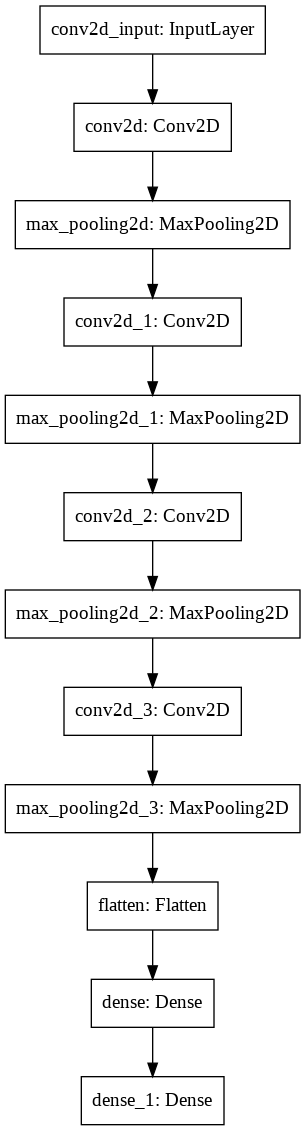
\includegraphics[width=5cm]{smc-best-model.png}
            \caption{The schematic diagram of two biological neurons.}\label{fig:neurons}
        \end{figure}

        \section{Benign and Malignant}  % -- All the images on this section starts with the name Scratch Benign and Malignant (sbm-xxxxx.png) 

    % --------------------------------------------------------------------
    
    \chapter{Pre-Trained CNN}

    % --------------------------------------------------------------------

    \chapter{Baseline Abnormality detection in mammography}

    % --------------------------------------------------------------------

    \chapter{Ensemble of Neural Networks}
    \section{Examples of Predictions}

    % --------------------------------------------------------------------

\end{document}